\chapterimage{images/kotlin/kotlinprogramminglanguage.png}

\chapter{Hello Kotlin}
In this chapter we will cover some of the fundamentals of the basic Kotlin language.
It is not meant to be an exhaustive overview and you will find none or very little code examples.
The examples used can be found in the references spread around this chapter.

\section{Kotlin vs. Java}

Kotlin was created with Java developers in mind, and with IntelliJ as its main development IDE.
There are several resources on what Kotlin's advantages are over Java.
Maybe it is a good idea to have a look in the Kotlin documentation and see what they are telling.

Go to this link: \url{https://kotlinlang.org/docs/reference/comparison-to-java.html}

The most important differences for this lesson are:

\begin{enumerate}
	\item Kotlin is null safe, which means that we deal with possible null situations in compile time, to prevent execution time exceptions.
		We need to explicitly specify that an object can be null, and then check its nullity before	using it.
	\item As many other modern languages, it uses many concepts from functional programming, such as lambda expressions, to solve some problems in a much easier way.
		This was not possible in the Java-version of Android (at least not without the necessary extra libraries).
	\item It makes use of extension functions: this means we can extend any class with new features even if we don’t have access to the source code.
\end{enumerate}

If you need a refresher regarding the advanced Java concepts, we provide a small list explaining them (not in detail).

\begin{description}
	\item[Raw Type] Raw types refer to using a generic type without specifying a type parameter.
		For example, \texttt{List} is a raw type, while \texttt{List<String>} is a parameterized type.
		When generics were introduced in \gls{jdk} 1.5, raw types were retained only to maintain backwards compatibility with older versions of Java.
	\item[Checked Exception]: are the exceptions that are checked at compile time in Java.
		If some code within a method throws a checked exception, then the method must either handle the exception or it must specify the exception using throws keyword.
	\item[Unchecked Exception] Unchecked are the exceptions that are not checked at compiled time.
	\item[Lambda expression] Provide a clear and concise way to represent one method interface using an expression.
For a good introduction see \url{https://docs.oracle.com/javase/tutorial/java/javaOO/lambdaexpressions.html}
\end{description}

\section{Executing Kotling without Android}

You can use \url{try.kotlinlang.org} to test Kotlin and some other simple examples without the need of a real project.
You could also use the \gls{repl} that comes bundled with the Kotlin plugin.
You will find it in Tools $\rightarrow$ Kotlin $\rightarrow$ Kotlin \gls{repl}.

\section{Classes}
The full description of classes can be found in this link \url{https://kotlinlang.org/docs/reference/classes.html}.
This section only contains some pointers which you should not forget when programming.

\subsection{Inheritance}
By default, a class always extends from Any (similar to Java Object), but we can extend any other classes.
Note however: Any is not  equals to the java.lang.Object; in particular, it does not have any members other than equals(), hashCode() and toString().
Classes are closed by default (final), so we can only extend a class if it’s explicitly declared as open or abstract.

\section{Functions}
Functions in Kotlin always return a value.
So if you don’t specify a return value, it will return Unit.
Unit is similar to void in Java, though this is in fact an object.
You can, of course, specify any type as a return value.

Note that semicolons are not  necessary, and it’s a good practice to avoid them (the IDE will warn you).

You can use template expressions directly in your strings by prefixing with \$.
This will make it easy to write complex strings based on static and variable parts.

\section{Exercises }
In this series of exercises we are going to cover the \gls{solid} design pattern and we will illustrate them with Kotlin code.
Although the focus of these exercises is not the theory about these principles, we expect of course that you will apply these principles in the next chapters.
You can find the code examples also in GitHub: \url{https://github.com/eothein/SOLID/tree/master}

If for some reason the authors  have forgotten to apply them in the examples, do not hesitate to  harass and try to disconcert us with with questions and challenges regarding these exercises or examples.


\subsection{\gls{solid} code}
\gls{solid} is an acronym for the first five object-oriented design \gls{ood} principles by Robert C. Martin.

These principles, when combined together, make it easy for a programmer to develop software that are easy to maintain and extend.
They also make it easy for developers to easily refactor code and are also a part of the agile or adaptive software development.

We will list these principles in short:

\begin{description}
	\item[S] Single responsibility principle
	\item[O] Open-closed principle
	\item[L] Liskov substitution principle
	\item[I] Interface segregation principle
	\item[D] Dependency Inversion Principle
\end{description}

The following subsection describes the principles in more detail.
The figures have been retrieved from \cite{Devilla2009}, while the explanation and example come from \cite{OODesigncom2018,Janssen2018,Laanaya2016,Lipovetskii2017}

\subsubsection{Single responsibility principle }
\begin{framed}
The \gls{srp} states that a class should have one and only one reason to change, meaning that a class should have only one job.	
\end{framed}

\begin{figure}
	\centering
	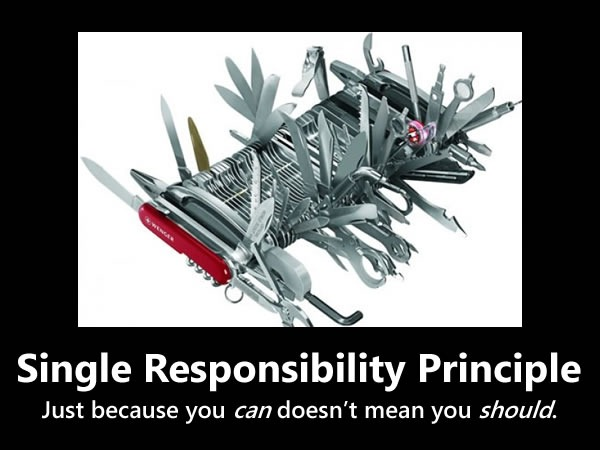
\includegraphics[width=0.8\textwidth]{images/kotlin/SRP.jpg}
	\caption{The “S” in \gls{solid} is for Single Responsibility Principle, which states that every object should have a single responsibility and that all of its services should be aligned with that responsibility.
		“Responsibility” is defined as “a reason to change”}
	\label{fir:SRP}
\end{figure}

As an example, consider an application that compiles and prints a book.
Such an object can be changed for two reasons:
\begin{inparaenum}[(i)]
	\item the content of the report can change and
	\item the format of the report can change.
\end{inparaenum}
 These two things change for very different causes; one substantive, and one cosmetic.
The single responsibility principle says that these two aspects of the problem are really two separate responsibilities, and should therefore be in separate classes or modules.
It would be a bad design to couple two things that change for different reasons at different times.

\begin{exercise}
Let's have a look at the code in listing \ref{code:KotlinSRPBook}.
This is a simple implementation in Kotlin which could implement the requirements listed above, although it does not abide the \gls{srp}.
Write down for yourself why this is the case and make an implementation that does abide the \gls{srp}.
\end{exercise}

\lstinputlisting[language=Kotlin, caption={The Kotlin code describing a book.
This source code does not abide the Single Responsibility Principle.}, label=code:KotlinSRPBook]{srccode/kotlin/book.kt}

\subsubsection{Open-Closed Principle}

\begin{figure}
	\centering
	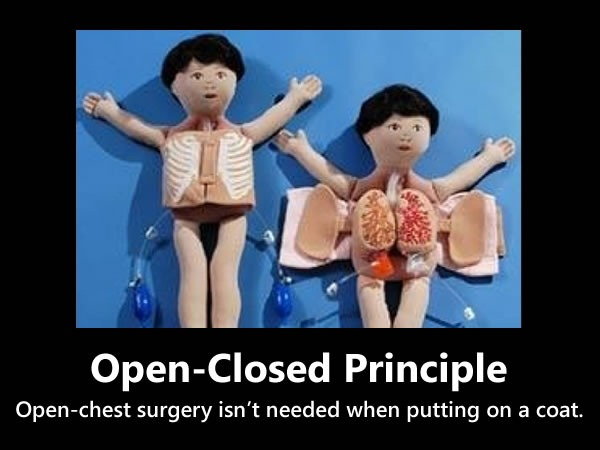
\includegraphics[width=0.8\textwidth]{images/kotlin/OCP.jpg}
	\caption{The “O” in \gls{solid} is for \gls{ocp}, which states that software entities such as classes, modules, functions and so on should be open for extension but closed for modification.
		The idea is that it’s often better to make changes to things like classes by adding to or building on top of them (using mechanisms like subclassing or polymorphism) rather than modifying their code.}
	\label{fir:OCP}
\end{figure}


\begin{framed}
	The \gls{ocp} states that software entities (classes, modules, functions, etc.) should be open for extension, but closed for modification, i.e. such an entity can allow its behaviour to be extended without modifying its source code.
\end{framed}

The \gls{ocp} is tightly coupled with the Single \gls{srp}.
If we design a class with SRP in mind, it is very likely that we also respect OCP or that little work is required to meet both, and vice versa.
Think about the following example: let’s say that we’ve got a Rectangle class with s a width and a height and we want to build an application that can calculate the total area of a collection of rectangles.
See the rectangle code in \ref{code:KotlinOCPRectangle}.

\lstinputlisting[language=Kotlin, caption={The source code describing a rectangle.}, label=code:KotlinOCPRectangle]{srccode/kotlin/Rectangle.kt}

That’s not a problem for us.
We learned in school that the area of a rectangle is its width multiplied with its height and we come up with the solution provided in TODO REF

\lstinputlisting[language=Kotlin, caption={The code to calculate the area of a rectangle.}, label=code:KotlinOCPArea]{srccode/kotlin/AreaCalculator.kt}


Now write down what the problem is with this solution.
Say you now also need to calculate the area of a circle.
What things do you need to adjust? 

\begin{exercise}
	Think about the things you have written and create the code which implements the \gls{srp} and the  \gls{ocp} correctly. 
\end{exercise}

\subsubsection{Liskov Substitution Principle}


\begin{framed}
	The \gls{lsp} states that functions that use pointers or references to base classes must be able to use objects of derived classes without knowing it.
\end{framed}

\begin{figure}
	\centering
	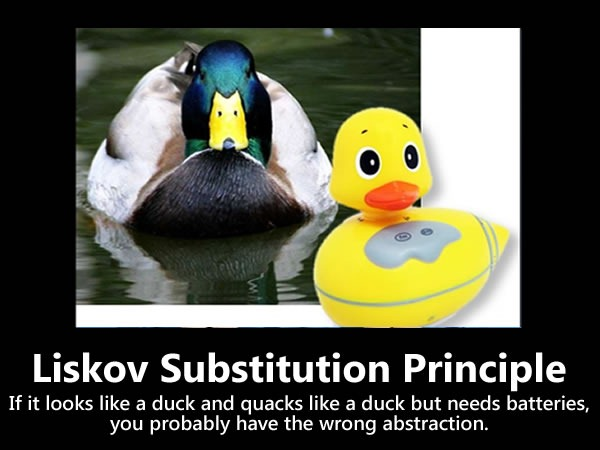
\includegraphics[width=0.8\textwidth]{images/kotlin/LSP.jpg}
	\caption{The “L” in \gls{solid} is for \gls{lsp} which states that subclases should be substitutable for the classes from which they were derived.
		For example, if MySubclass is a subclass of MyClass, you should be able to replace MyClass with MySubclass without bunging up the program.}
	\label{fir:LSP}
\end{figure}

A great example illustrating \gls{lsp}  was how sometimes something that sounds right in natural language doesn't quite work in code.

In mathematics, a Square is a Rectangle.
Indeed it is a specialization of a rectangle.
The "is a" makes you want to model this with inheritance.
However if in code you made Square derive from Rectangle, then a Square should be usable anywhere you expect a Rectangle.
This makes for some strange behavior which needs to override of functions which normally should not be overwritten.
See the code in listing \ref{code:KotlinLSP}.

\lstinputlisting[language=Kotlin, caption={Implementation of a square by inheriting from Rectangle}, label=code:KotlinLSP]{srccode/kotlin/Square.kt}

Imagine you had SetWidth and SetHeight methods on your Rectangle base class; this seems perfectly logical.
However if your Rectangle reference pointed to a Square, then SetWidth and SetHeight doesn't make sense because setting one would change the other to match it.
In this case Square fails the Liskov Substitution Test with Rectangle and the abstraction of having Square inherit from Rectangle is a bad one.

\begin{exercise}
	Make an implementation of the Square and Rectangle which implements the \gls{srp},  \gls{ocp}  and the \gls{lsp} correctly. 
\end{exercise}

\subsubsection{Interface Segregation Principle}

\begin{framed}
	The \gls{isp} states that no client should be forced to depend on methods it does not use.
	ISP splits interfaces that are very large into smaller and more specific ones so that clients will only have to know about the methods that are of interest to them.
\end{framed}

\begin{figure}
	\centering
	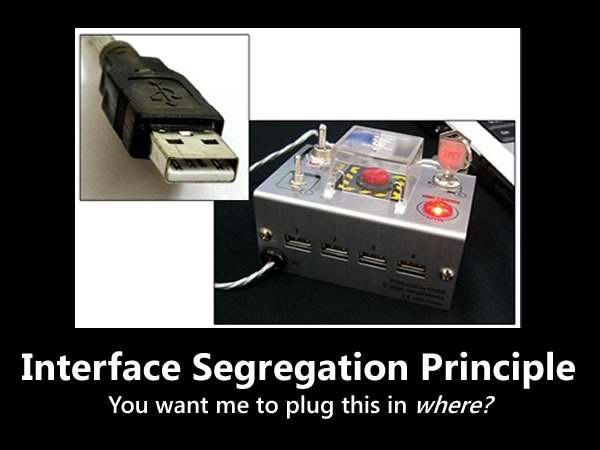
\includegraphics[width=0.8\textwidth]{images/kotlin/ISP.jpg}
	\caption{The “I” in SOLID is for \gls{isp}, which states that clients should not be forced to depend on methods they don’t use.
		If a class exposes so many members that those members can be broken down into groups that serve different clients that don’t use members from the other groups, you should think about exposing those member groups as separate interfaces.}
	\label{fir:lsp}
\end{figure}

What the Interface Segregation Principle says is that your interface should not be bloated with methods that implementing classes don’t require.
For such interfaces, also called “fat interfaces”, implementing classes are unnecessarily forced to provide implementations (dummy/empty) even for those methods that they don’t need.
In addition, the implementing classes are subject to change when the interface changes.
An addition of a method or change to a method signature requires modifying all the implementation classes even if some of them don’t use the method.

See the following implementation.
We have a component which should work on both an Android device and on a Desktop. 

\lstinputlisting[language=Kotlin, caption={Interface for the component.}, label=code:KotlinComponent]{srccode/kotlin/Component.kt}

\lstinputlisting[language=Kotlin, caption={The desktop component.}, label=code:KotlinDesktop]{srccode/kotlin/DesktopComponent.kt}

\lstinputlisting[language=Kotlin, caption={The Android component.}, label=code:KotlinAndroid]{srccode/kotlin/AndroidComponent.kt}

\begin{exercise}
	Redesign the Component stack to that it satisfies \gls{isp}.
\end{exercise}


\subsubsection{Dependency Inversion Principle}

\begin{framed}
	The \gls{dip} states that:
	\begin{itemize}
		\item High-level modules should not depend on low-level modules.
			Both should depend on abstractions.
		\item Abstractions should not depend on details.
			Details should depend on abstractions.
	\end{itemize}
\end{framed}

An important detail of this definition is that high-level and low-level modules depend on the abstraction.
The design principle does not just change the direction of the dependency, as you might have expected when you read its name for the first time.
It splits the dependency between the high-level and low-level modules by introducing an abstraction between them.
So in the end, you get two dependencies:

Below is an example which violates the Dependency Inversion Principle.
We have the manager class  (see \ref{code:KotlinManager}) which is a high level class, and the low level class called Worker (see \ref{code:KotlinWorker}).

\lstinputlisting[language=Kotlin, caption={The manager class}, label=code:KotlinManager]{srccode/kotlin/Manager.kt}

\lstinputlisting[language=Kotlin, caption={The Worker  class.}, label=code:KotlinWorker]{srccode/kotlin/Worker.kt}

We need to add a new module to our application to model the changes in the company structure determined by the employment of new specialized workers.
We created a new class SuperWorker for this.

Let's assume the Manager class is quite complex, containing very complex logic.
And now we have to change it in order to introduce the new SuperWorker.
Let's see the disadvantages:

\begin{enumerate}
	\item we have to change the Manager class (remember it is a complex one and this will involve time and effort to make the changes).
	\item some of the current functionality from the manager class might be affected.
	\item the unit testing should be redone.
\end{enumerate}

All those problems could take a lot of time to be solved and they might induce new errors in the old functionlity.
The situation would be different if the application had been designed following the \gls{dip}.
It means we redesign the manager class, implement an IWorker interface and the Worker class implementing the IWorker interface.
When we need to add the SuperWorker class all we have to do is implement the IWorker interface for it.
No additional changes in the existing classes.

\begin{exercise}
	Make the changes to the implementation and describe why this is better.
	Does your solution address the problems mentioned above? 
\end{exercise}

\begin{figure}
	\centering
	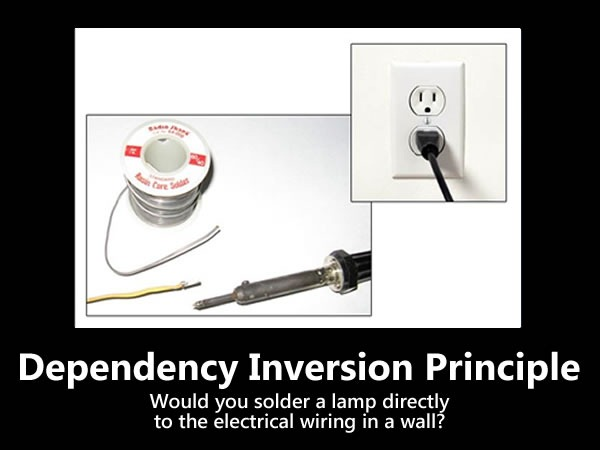
\includegraphics[width=0.8\textwidth]{images/kotlin/DIP.jpg}
	\caption{The “D” in SOLID is for \gls{dip}, which states that high-level modules shouldn’t depend on low-level modules, but both should depend on shared abstractions.
		In addition, abstractions should not depend on details – instead, details should depend on abstractions.}
	\label{fir:dsp}
\end{figure}


